\section{Robot Localisation in Vineyard Pruning}
\label{sec:vineyard-pruning}
Pruning typically occurs in the dormant season (winter), which introduces a unique robot localisation challenge in the form of geometric sparsity and the lack of distinctive visual features caused by the absence of foliage~\cite{youOpticalFlowbasedBranch2022}. The environment consists of thin, bare branches that provide a low density of sensor returns and few distinctive visual textures for cameras to localise on~\cite{youOpticalFlowbasedBranch2022}. Without leaves to block the view, sensors often pick up background clutter from the sky or neighbouring rows, complicating foreground segmentation~\cite{youOpticalFlowbasedBranch2022}. The following analysis details the strategies used for spatial alignment with vines, specifically in the context of robotic pruning platforms.

\subsection{Spatial Alignment Modalities for Pruning Vines}
\label{subsec:spatial-alignment-modalities}
While traditional passive vision remains the baseline for high-resolution 3D modelling, it faces significant geometric and environmental hurdles. To address the ill-conditioned configurations of binocular systems, specifically when linear canes align with the stereo baseline, Botterill et al. employ a trinocular rig consisting of three 1.3-megapixel cameras arranged in a triangular configuration, housed within a vine-straddling mobile platform (\cref{fig:botterilRobot})~\cite{botterillRobotSystemPruning2017}. This allows for the dynamic selection of the mathematically optimal camera pair for specific cane segments, a level of geometric robustness that passive binocular systems lack.

\begin{figure}[ht]
    \centering
    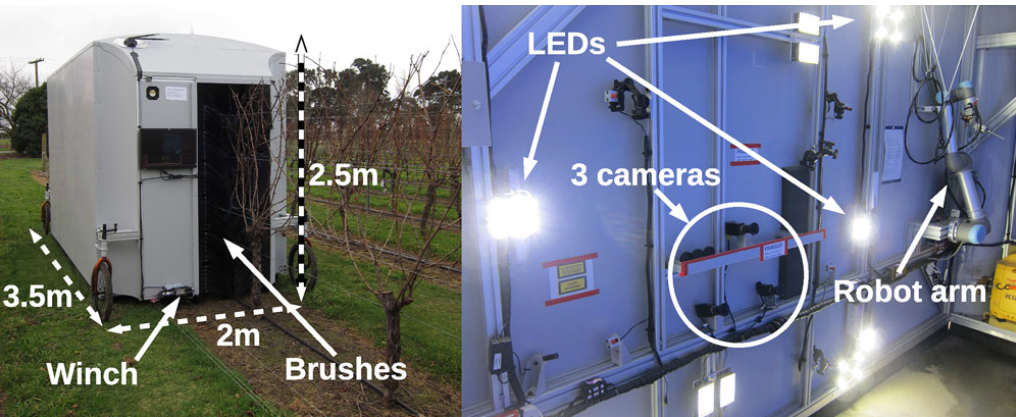
\includegraphics[width=0.85\linewidth]{2-background/figures/botterilRobot.png}
    \caption{The vine-straddling mobile platform developed by Botterill et al., shown from outside (left) and inside (right). The enclosed structure shields the workspace from ambient sunlight, while the interior houses the trinocular camera array, high-intensity LED illumination, a six degree-of-freedom robot arm, and an on-board PC for real-time processing \protect\cite{botterillRobotSystemPruning2017}.}
    \label{fig:botterilRobot}
\end{figure}

However, even optimised trinocular systems remain vulnerable to outdoor lighting variability. This necessitates a shift toward active sensing, either through illumination or direct range-finding. The Bumblebee platform integrates an active light stereo camera system to generate dual point clouds, which are registered via transformation matrices and refined with the Iterative Closest Point (ICP) algorithm to maintain invariance against ambient shadows~\cite{silwalBumblebeePath2022}. Active-light camera designs of this type also improve robustness to varying outdoor illumination more broadly~\cite{silwalRobustIlluminationInvariantCamera2021}. In contrast, Felicetti et al. bypass the lighting and correspondence problem entirely by utilising downward-facing 3D LiDAR~\cite{felicettiTractorMountedGrapevine2025}. By applying a minimalist depth-thresholding algorithm within a specific range ($D_{min}$ to $D_{max}$, typically 250--500 mm), this approach sacrifices the fine-grained topological understanding provided by Botterill's trinocular rig in favour of throughput, processing a vine in just 7.3 seconds~\cite{felicettiTractorMountedGrapevine2025, botterillRobotSystemPruning2017}.

The data processing pipelines of these approaches are also vastly different. Botterill et al. prioritise spatial stability for robotic manipulation through a heavy incremental bundle adjustment pipeline. By utilising the \textit{g2o} graph optimisation framework and robust Pseudo-Huber cost functions to penalise large residuals, they achieve trajectory errors below 1\%, though at a higher computational cost~\cite{botterillRobotSystemPruning2017}. Recent work, however, suggests that such global optimisation may be unnecessary for effective pruning. The Archie Jnr platform employs deep panoptic segmentation (Detectron2) to identify cane structures and nodes, enabling autonomous vine assessment for three-cane pruning decisions~\cite{williamsArchieJnrRobotic2024}. Separately, Hizatate et al. propose a system combining RGB-D cameras with a 6-DoF manipulator, estimating grapevine structures to identify pruning points with 62\% accuracy~\cite{hizatateDevelopmentRobotPruning2025}.

By registering segmentation masks with depth data, these neural architectures occupy the middle ground between the high-fidelity reconstruction of Botterill et al. and the high-speed approach of Felicetti et al. Williams et al. demonstrate that Archie Jnr successfully prunes 71.1\% of required canes across real-world vineyard trials~\cite{williamsArchieJnrRobotic2024}, while Bumblebee's active lighting and Faster R-CNN bud detection pipeline provides the precision required for dormant-season cane identification~\cite{silwalBumblebeePath2022}. The trinocular approach provides the most detailed 3D map for precise spur pruning, but the integration of active illumination and semantic segmentation offers a more computationally viable path toward commercial field speeds.

\begin{table}[h]
\centering
\caption{Comparison of Perception Modalities for Vineyard Pruning}
\label{tab:perception}
\begin{tabularx}{\textwidth}{|X|l|l|}
\hline
\textbf{System} & \textbf{Modality} & \textbf{Key Metric} \\ \hline
Botterill et al.~\cite{botterillRobotSystemPruning2017} & Trinocular Stereo & 120 s/vine \\ \hline
Bumblebee~\cite{silwalBumblebeePath2022} & Active Light Stereo & 137 s/vine \\ \hline
Felicetti et al.~\cite{felicettiTractorMountedGrapevine2025} & 3D LiDAR & 7.3 s/vine \\ \hline
Archie Jnr~\cite{williamsArchieJnrRobotic2024} & RGB-D + Panoptic Seg. & 71.1\% prune success \\ \hline
Hizatate et al.~\cite{hizatateDevelopmentRobotPruning2025} & RGB-D + 6-DoF Arm & 62\% accuracy \\ \hline
\end{tabularx}
\end{table}

\subsection{Summary}
\label{subsec:vineyard-pruning-summary}

Existing robotic pruning platforms demonstrate that millimetre-level spatial alignment is achievable, but they share a common architectural assumption: perception, planning, and execution are tightly coupled within a single real-time pipeline. The UCVision approach departs from this assumption by decoupling the data-collection phase from the intervention phase, generating a high-fidelity 3D Gaussian Splatting model offline before any manipulation is attempted. This decoupling introduces a spatial synchronisation problem that no existing pruning platform directly addresses: given a pre-computed pruning plan expressed in the coordinate frame of an offline 3D model, how can a robot executing that plan achieve the centimetre-level registration accuracy necessary to transfer planned cut-points to physical vine structures? This gap motivates the contributions of \cref{chap:SLAM} and \cref{chap:precise-alignment}.

